\section{Simulation d'un système de freinage sans ABS}
Durant la pratique des travaux sur VHDL-AMS il est demandé aux étudiants de réaliser et d'instancier étapes par étapes les différentes partie d'un système de freinage d'une voiture. Pour la réalisation du travail nous avons travailler avec le logiciel ModelSim et un éditeur de texte pour venir rédiger, en VHDL, les différentes instances du véhicule jusqu'à l'intégration de l'ABS.

\begin{figure}[h]
    \centering
    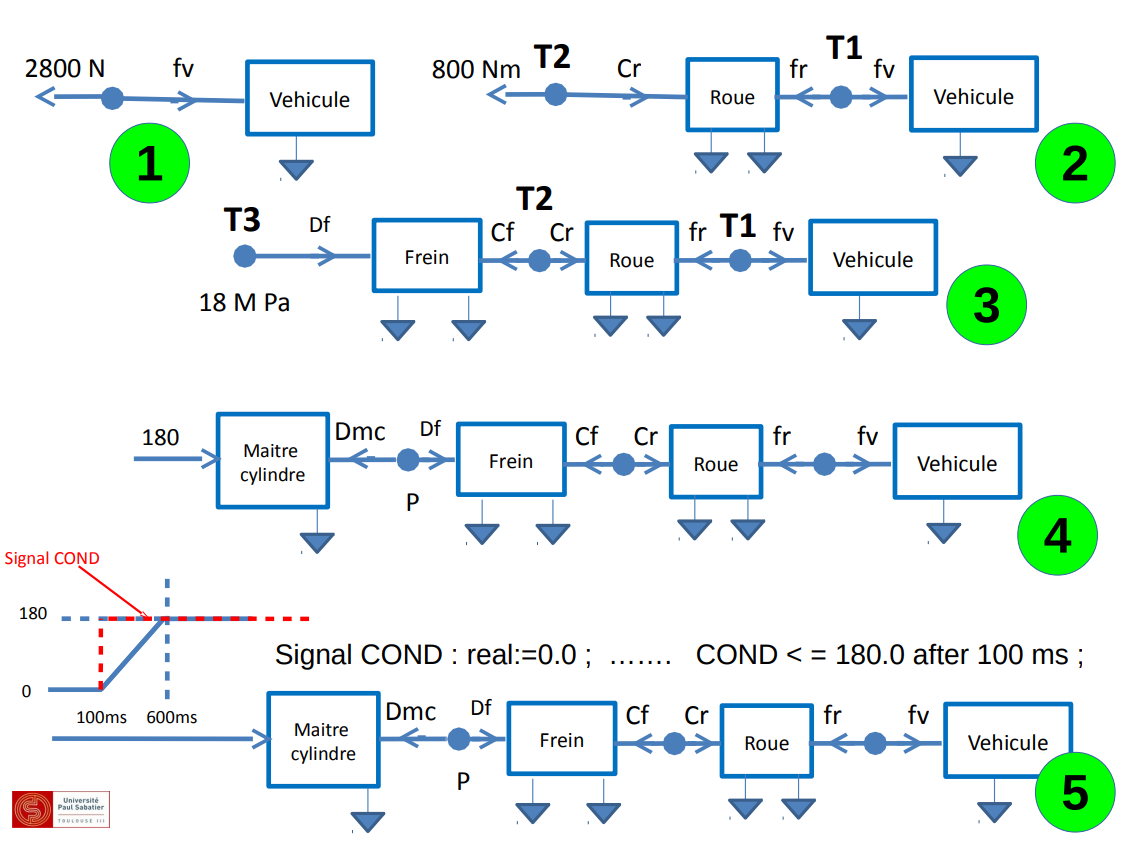
\includegraphics[width=\textwidth]{images/etapes.png}
    \caption{Implémentation des différentes parties du système de freinage d'une voiture}
\end{figure}

Il est demandé d'instancier étapes par étapes différents blocs avec leurs terminaux coresspondants, comme indiqué dans le powerpoint de présentation du TP.

\newpage

\subsection{Analyse instanciation véhicule }
Dans cette première partie nous devons instancié le véhicule fournit dans les fichiers du projet. Sur la Figure 2 on peut voir le schéma bloc qu'il faut instancier et décrire par son entitée en VHDL-AMS.

\begin{figure}[h]
    \centering
    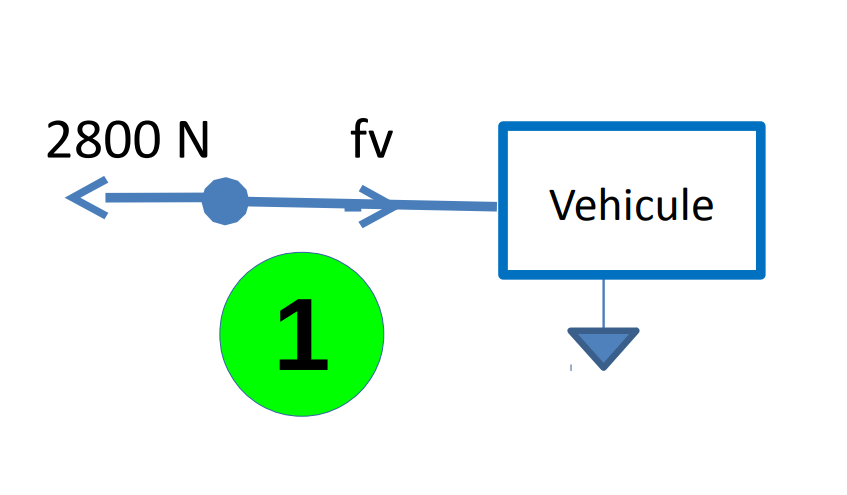
\includegraphics[width=0.5\textwidth]{images/un.png}
    \caption{Instanciation du véhicule avec son terminal}
\end{figure}

Dans l'entitée du véhicule nous avons donc à définir certaines quantités qui va nous permettra de résoudre certaines équations. Les paramètres d'entrées de notre première équation sont les suivants :\\

\begin{itemize}
        \item $m        \rightarrow$ Masse véhicule.
        \item $Cx       \rightarrow$ Coéfficient aérodynamique.
        \item $S        \rightarrow$ Surface Frontale.
        \item $V\_init  \rightarrow$ Vitesse initiale du vehicule.
\end{itemize}

\begin{figure}[h]
    \centering
    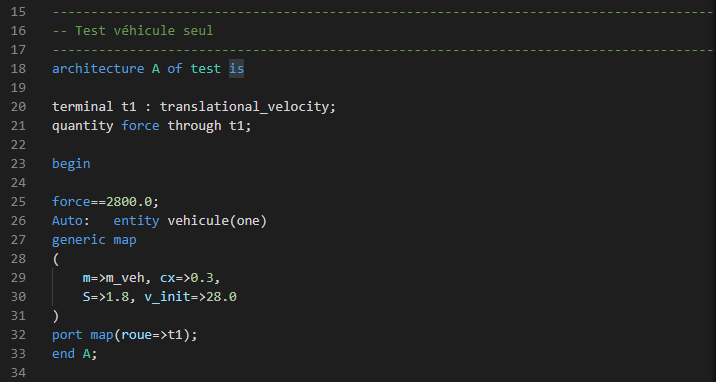
\includegraphics[width=\textwidth]{images/vehicule.png}
    \caption{Code VHDL Architecture A - Véhicule}
\end{figure}

Pour la première partie, véhicule il faudra mettre en place un terminal T1 ayant pour type "Translational\_velocity". Celui-ci sera plus tard rélié au Terminal "Roue", du même type, pour nous permettre la visualisation de la vitesse du véhicule.
\newpage
Avec l'aide du logiciel ModelSim nous pouvons simuler le temps de freinage nécessaire à l'arrêt du véhicule lorsqu'on lui applique une force de 2800 N au terminal T1.

\begin{figure}[h]
    \centering
    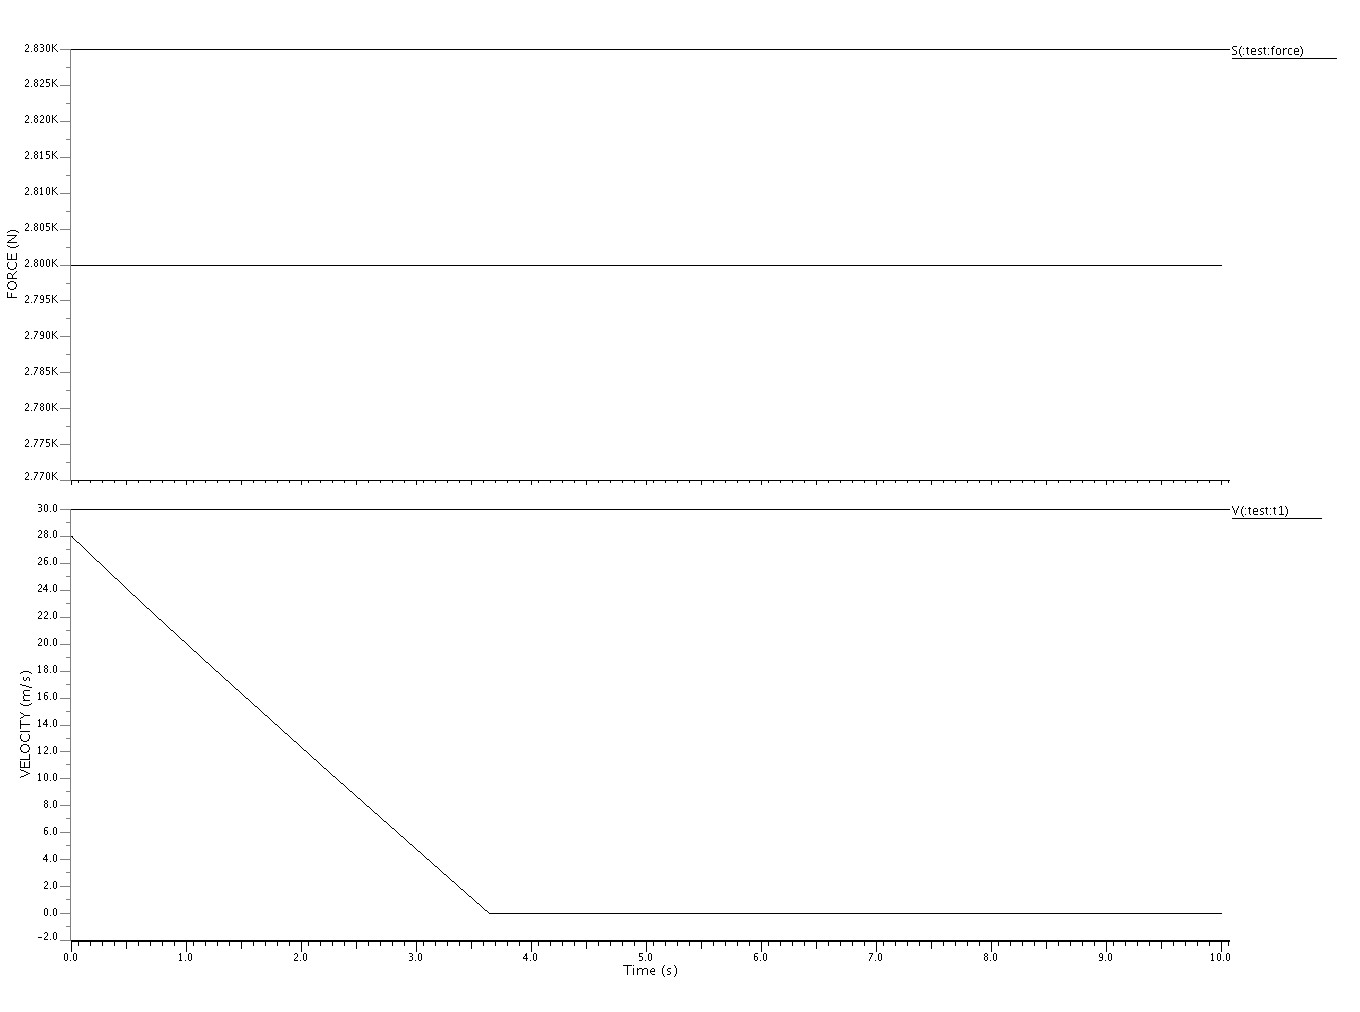
\includegraphics[width=\textwidth]{images/Instanciation_vehicule.jpg}
    \caption{Simulation Terminal T1 Force et Temps pour le freinage}
\end{figure}

\subsection{Analyse instanciation roue}

Dans cette seconde partie nous devons instancier la roue fournit dans les fichiers du projet. Sur la Figure 5 on peut voir le schéma bloc qu'il faut instancier et décrire par la suite son entitée en VHDL-AMS.

\begin{figure}[h]
    \centering
    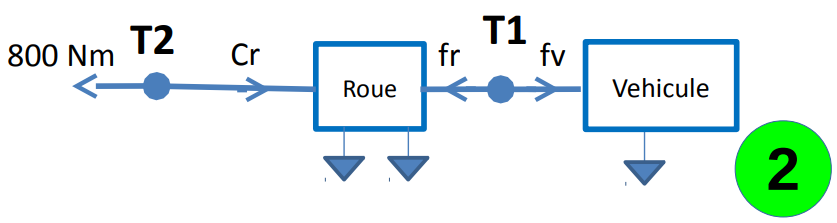
\includegraphics[width=0.7\textwidth]{images/deux.png}
    \caption{Instanciation du véhicule avec son terminal}
\end{figure}

\newpage

Une fois le véhicule instancié on nous demande d'ajouter le système "Roue". Dans cette partie on déclare en code la partie générique qui va nous permettre de résoudre l'équation suivante ayant pour entrées ces paramètres :\\
\begin{itemize}
    \item $route       \rightarrow$ Etat de la route (mouillée, seche).
    \item $m       \rightarrow$ Masse vehicule.
    \item $rR        \rightarrow$ Rayon de la roue.
    \item $IR  \rightarrow$ Inertie de la roue.
    \item $mu0_D \rightarrow$ Coéfficient adhérence sans glissement sur sol sec.
    \item $As \rightarrow$ Facteur de decroissance de l'adherence.
    \item $mu0_W \rightarrow$ Coéfficient adhérence sans glissement sur sol mouillé.
    \item $Vc \rightarrow$ Caracteristique de la surface.
\end{itemize}


Dans cette partie du code il y aura deux terminaux à instancier au niveau de la roue :\\

\begin{itemize}
    \item $veh  \rightarrow $ De type "translational\_velocity".
    \item $frein    \rightarrow $ De type "rotational\_velocity".
\end{itemize}

\begin{figure}[h]
    \centering
    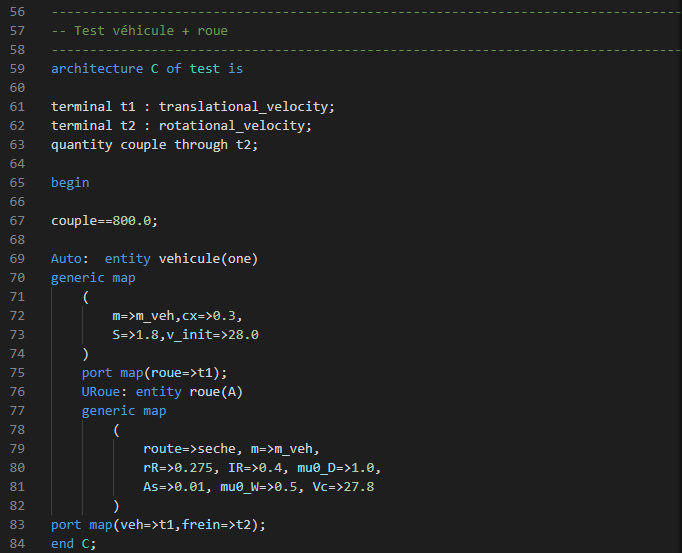
\includegraphics[width=\textwidth]{images/Roue.png}
    \caption{Code VHDL Architecture C - Roue}
\end{figure}

\newpage

Une fois la "Roue" implémentée on se retrouve sur ModelSim avec deux Terminaux, T2 étant le dernier terminal instancié qui représente le terminal d'entrée de "Roue" et T1 son Terminal de sortie. On observe grâce à ModelSim la vitesse rotationnelle de "Roue" ainsi que la vitesse du véhicule. On constate que la vitesse de "Roue" chute brusquement avant de réduire linéairement comme pour la vitesse du véhicule.

\begin{figure}[h]
    \centering
    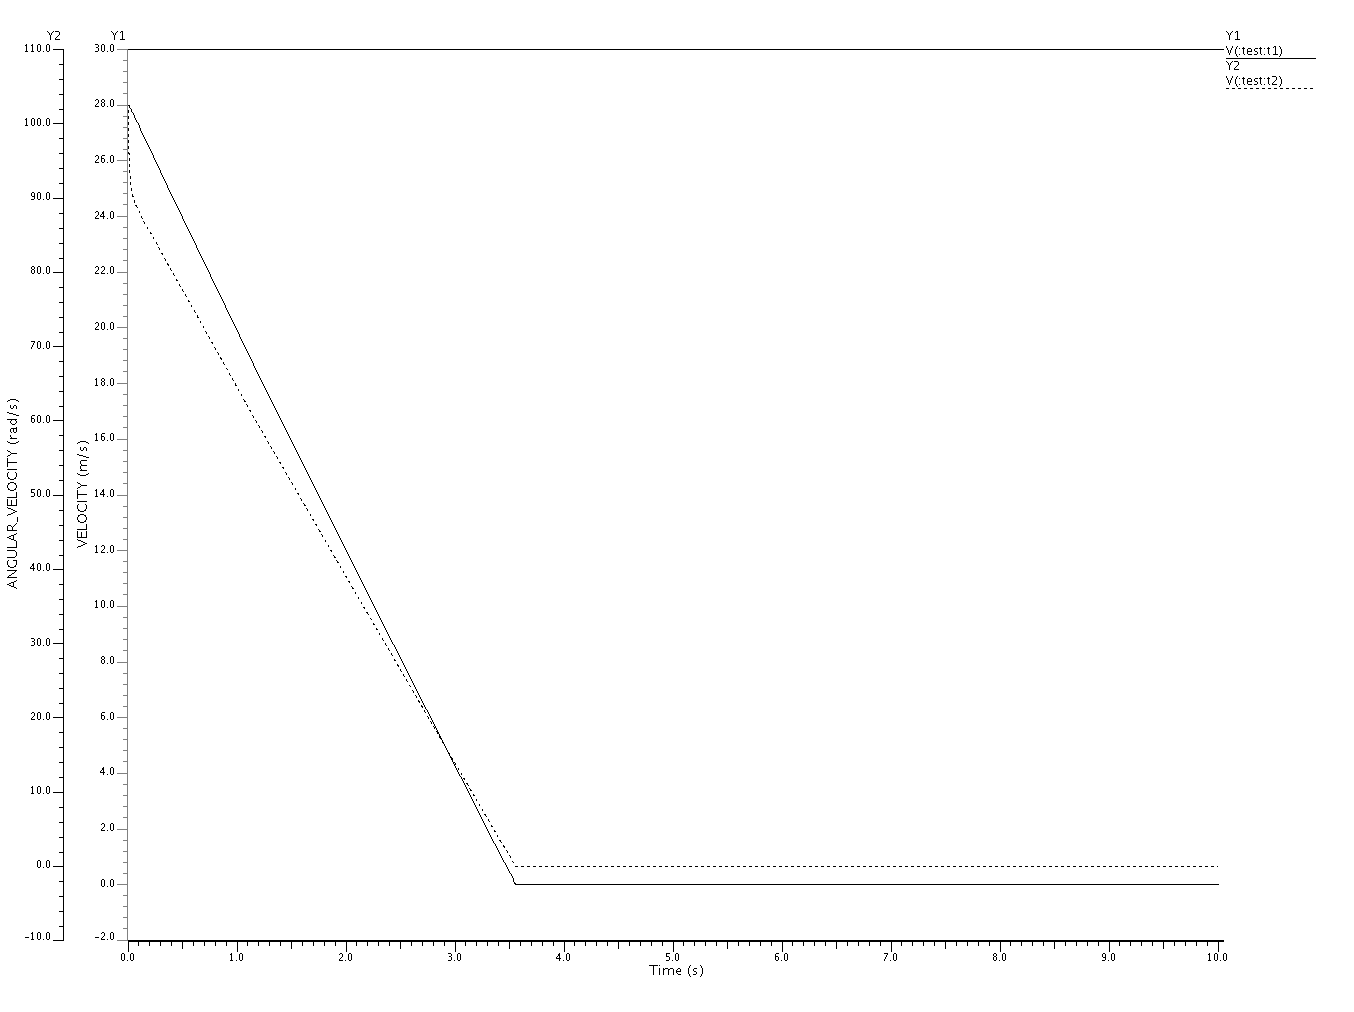
\includegraphics[width=\textwidth]{images/Frein.png}
    \caption{Simulation Terminal T2 et T1}
\end{figure}

\subsection{Analyse instanciation frein}

Dans la troisème partie du tp nous devons instancier le frein au terminal T2, fournit dans les fichiers du projet. Sur la Figure 8 on peut voir le schéma bloc qu'il faut instancier et décrire par la suite son entitée en VHDL-AMS.

\begin{figure}[h]
    \centering
    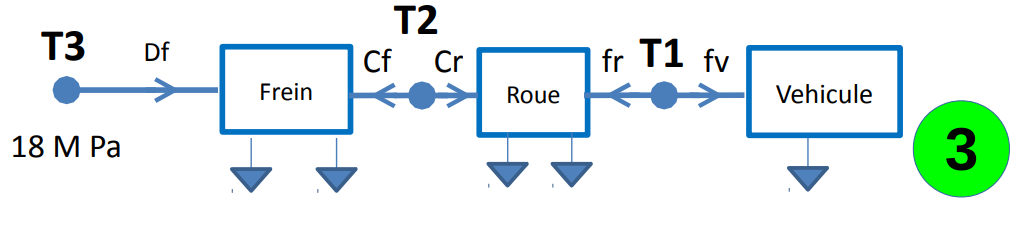
\includegraphics[width=0.7\textwidth]{images/trois.png}
    \caption{Instanciation du véhicule avec son terminal}
\end{figure}

\newpage 

Une fois le véhicule et la Roue instanciés on nous demande d'ajouter le système "Frein". Dans cette partie on déclare en code la partie générique suivante :\\
\begin{itemize}
    \item $coef_fric    \rightarrow$ Coéfficient de friction des plaquettes.
    \item $S    \rightarrow$ Surface piston = 10 cm2.
    \item $R   \rightarrow$ Rayon moyen du disque.
\end{itemize}

Dans cette partie du code il y aura deux terminaux à instancier au niveau de la du Frein :

\begin{itemize}
    \item $Roue    \rightarrow$ Type "rotational\_velocity".
    \item $MC    \rightarrow$ Type "fluidic" à l'entrée du Frein.
\end{itemize}

Dans cette nouvelle instance nous venons d'implémenter le "Frein" permettant l'obtention de la vitesse de rotation du disque dans le terminal 2 en fonction de la pression appliquée à son entrée. On définit une quantité de Pression (across) et un débit (Through) pour le nouveau Terminal. On vient ensuite fixer la valeur de pression à 18 MPa pour pouvoir résoudre l'équation.

\begin{figure}[h]
    \centering
    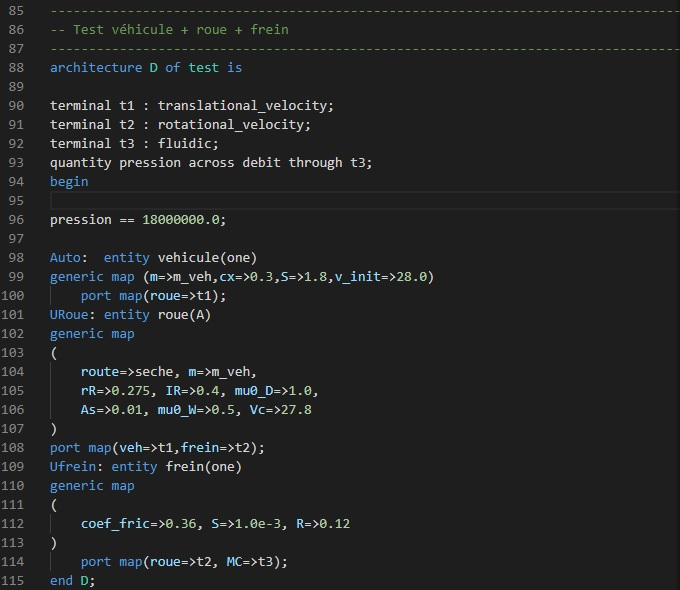
\includegraphics[width=0.95\textwidth]{images/Instanciation_frein.jpg}
    \caption{Code VHDL Architecture D - Roue et Frein}
\end{figure}
\newpage
Sur la figure 10 on peut observer grâce à la simulation que lorsque l'on applique une pression de 18 MPa au frein nous avons en sortie la vitesse qui décroit exactement comme à l'instanciation du véhicule ce qui nous permet de conclure que le frein est implémenté de la bonne manière.
\begin{figure}[h]
    \centering
    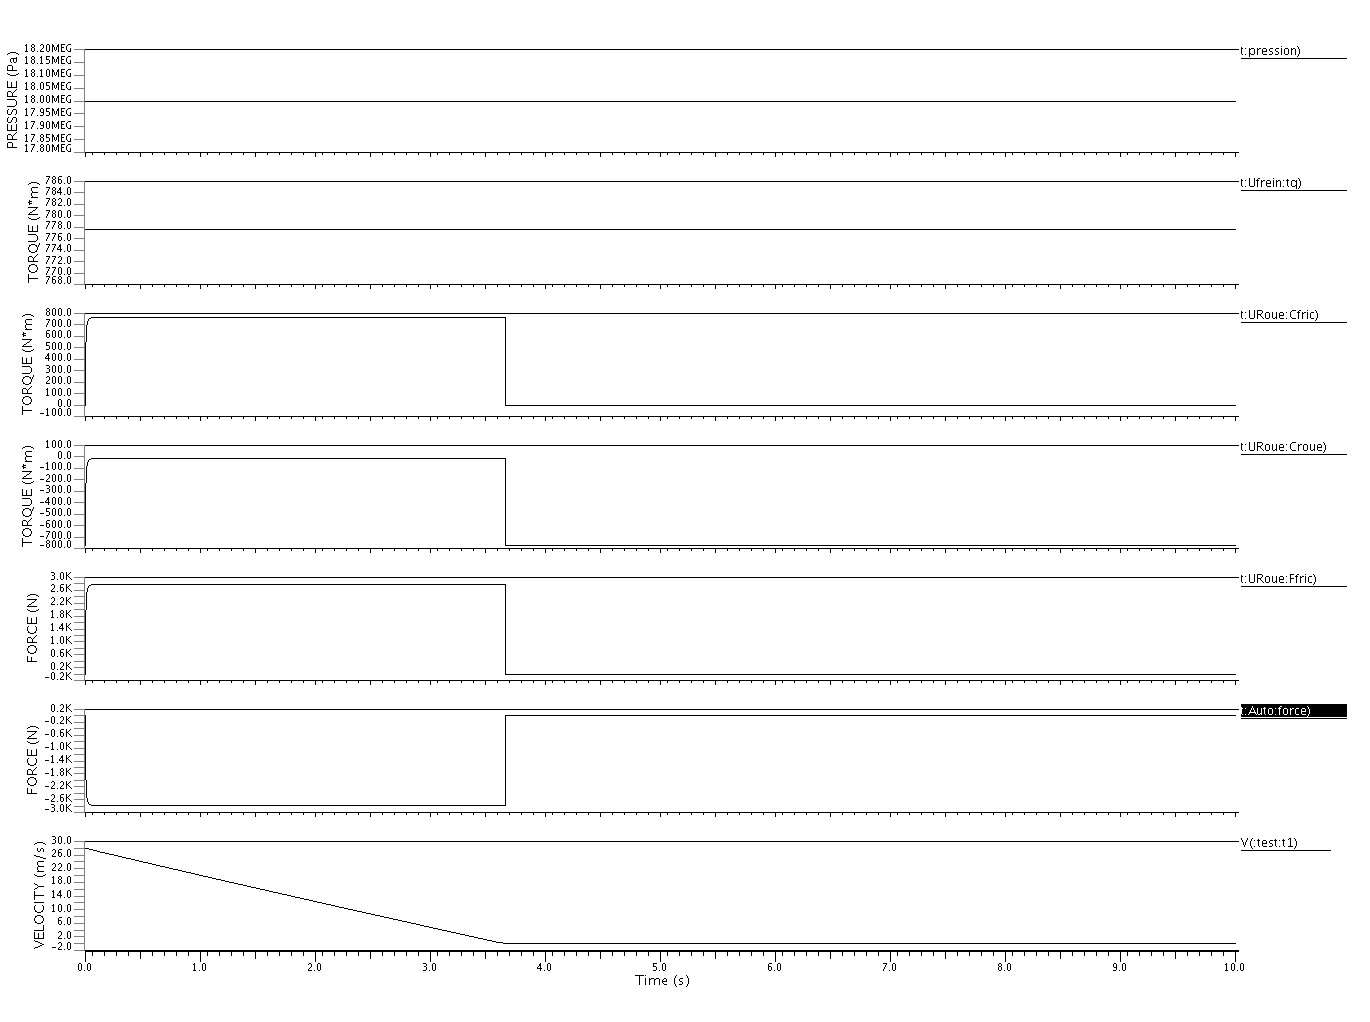
\includegraphics[width=\textwidth]{images/Instanciation_vehicule_roue_frein.jpg}
    \caption{Simulation Terminaux T3 T2 et T1}
\end{figure} 

\subsection{Analyse instanciation maître cylindre}
Dans la quatrième partie nous allons instancier le maître cylindre qui va permettre de transmettre la pression vers le terminal T3. Sur la Figure 11 on peut voir le schéma bloc qu'il faut instancier et décrire par la suite son entitée en VHDL-AMS.

\begin{figure}[h]
    \centering
    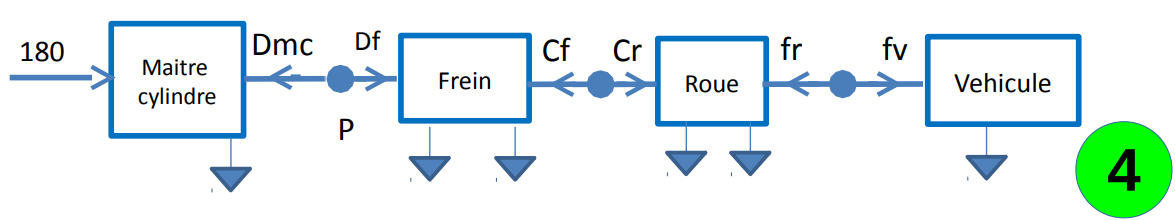
\includegraphics[width=0.85\textwidth]{images/quatre.png}
    \caption{Instanciation du véhicule avec son terminal}
\end{figure}
\newpage

Pour l'instanciation et la résolution du système maître cylindre  il sera nécessaire de compléter et de modifier le fichier fournit en TP. Dans cette partie on déclare en code la partie générique suivante :\\
\begin{itemize}
    \item $S    \rightarrow$ Coéfficient de friction des plaquettes.
    \item $S    \rightarrow$ Surface piston = 10 cm2.
\end{itemize}

Dans cette partie du code il y aura deux terminaux à instancier au niveau de la du Frein :

\begin{itemize}
    \item $Hyd    \rightarrow$ Type "fluidic" qui représente la pression en entrée du frein.
    \item $Force    \rightarrow$ Qui est une quantité réel exercée par le conducteur sur la pédale de frein.
\end{itemize}

\begin{figure}[h]
    \centering
    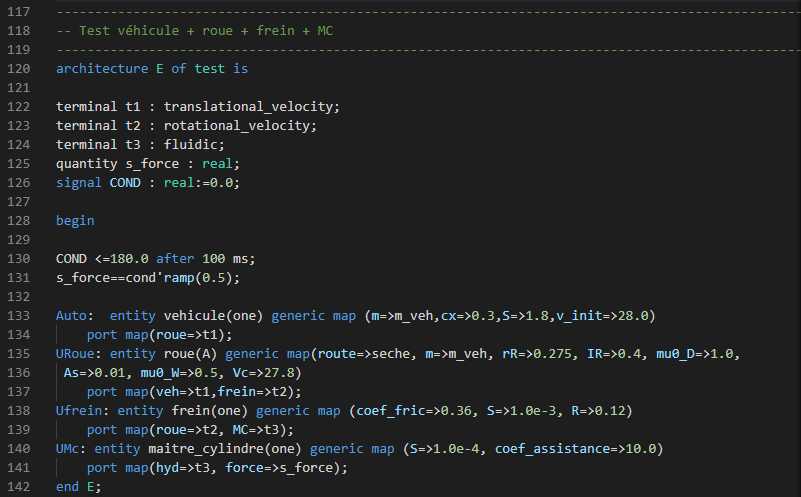
\includegraphics[width=0.95\textwidth]{images/MC.png}
    \caption{Code VHDL Architecture E - Maître cylindre}
\end{figure}
Dans cette nouvelle entité, maître cylindre, elle nous permet l'injection de la pression dans le frein en fonction de la force exercée par le conducteur sur la pédale de frein. Dnas ce nouveau cas Force étant un réel il est nécessaire de déclarer une quantité de type réel contrairement aux précédentes déclaration des Terminaux ultérieurs.
\newpage
\begin{figure}[h]
    \centering
    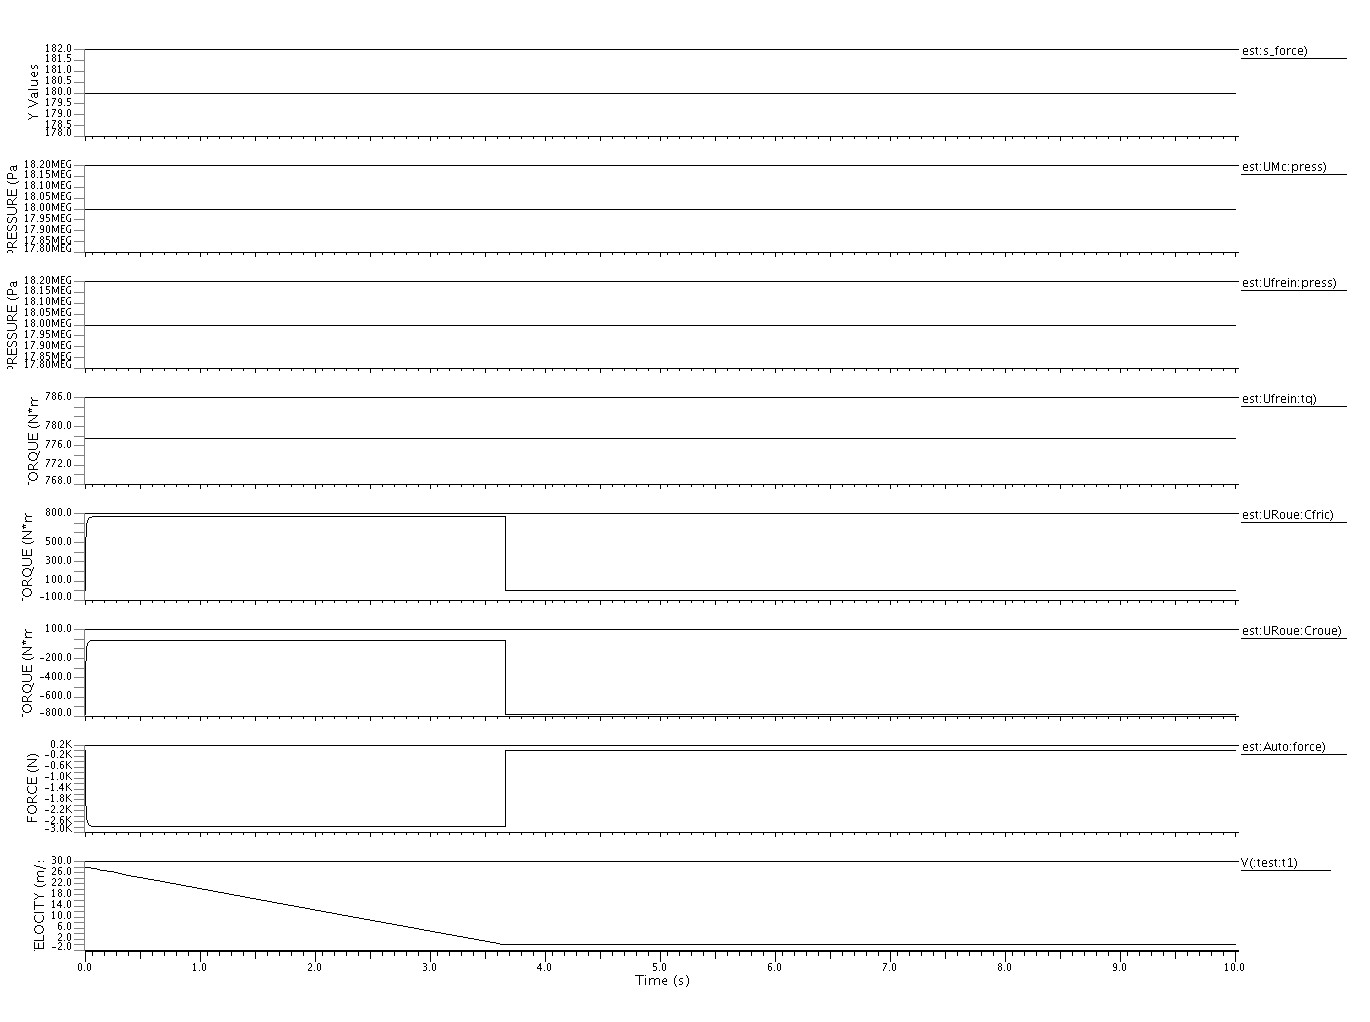
\includegraphics[width=\textwidth]{images/Instanciation_vehicule_roue_frein_Mc.jpg}
    \caption{Simulation du Terminal 4 - Maître cylindre}
\end{figure}
On constate avec l'outil de modélisation que lorsque nous appliquons une préssion de 180 N sur la pédale de frein nous obtenons un même temps de freinage et une même pression sur le frein que sur l'Implémentation précédente. Cette simulation nous permet de montrer la bonne implémentation de la partie correspondate au maître cylindre.

Pour la suite de cette partie on nous demande d'intégrer un temps de réaction du conducteur à notre entrée, permettant d'obtenir une simulation plus réaliste du système. Pour cela nous ajoutons un signal de type réel qui prendra la valeur de 180 N après 100 ms et par la suite affecter à ce signal une quatité de "Force" qui évoluera linéairement de 0 à 180 durant 500 ms.
\begin{figure}[h]
    \centering
    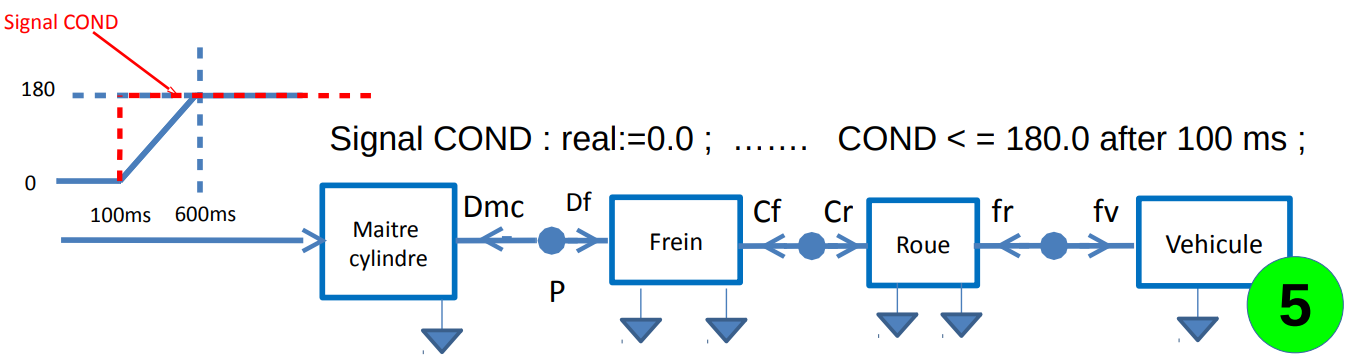
\includegraphics[width=\textwidth]{images/cinq.png}
    \caption{Intégration rampe au schéma bloc}
\end{figure}


\newpage
\begin{figure}[h]
    \centering
    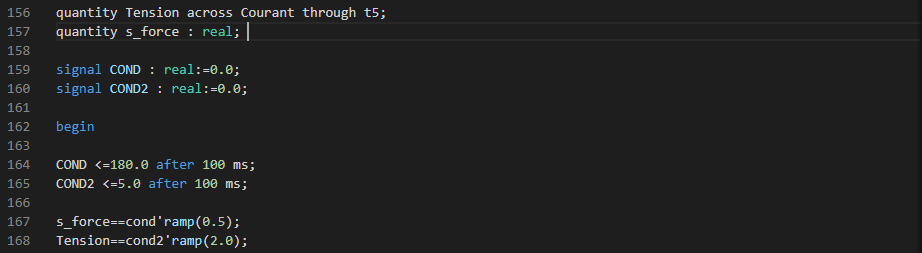
\includegraphics[width=\textwidth]{images/cond.png}
    \caption{Condition rampe entrée Maître cylibdre}
\end{figure}

En ajoutant cette condition nous pouvant oberser avec l'outil de simulation la nouvelle évolution de la vitesse du véhicule, qui maitenant, ne décroit plus linéairement. On constate que le véhicule met plus de temps pour freiner entièrement son déplacement, ce qui peut être expliqué du fait que tant que la force maximum du frein n'est pas appliquée le temps de freinage sera plus long.

\begin{figure}[h]
    \centering
    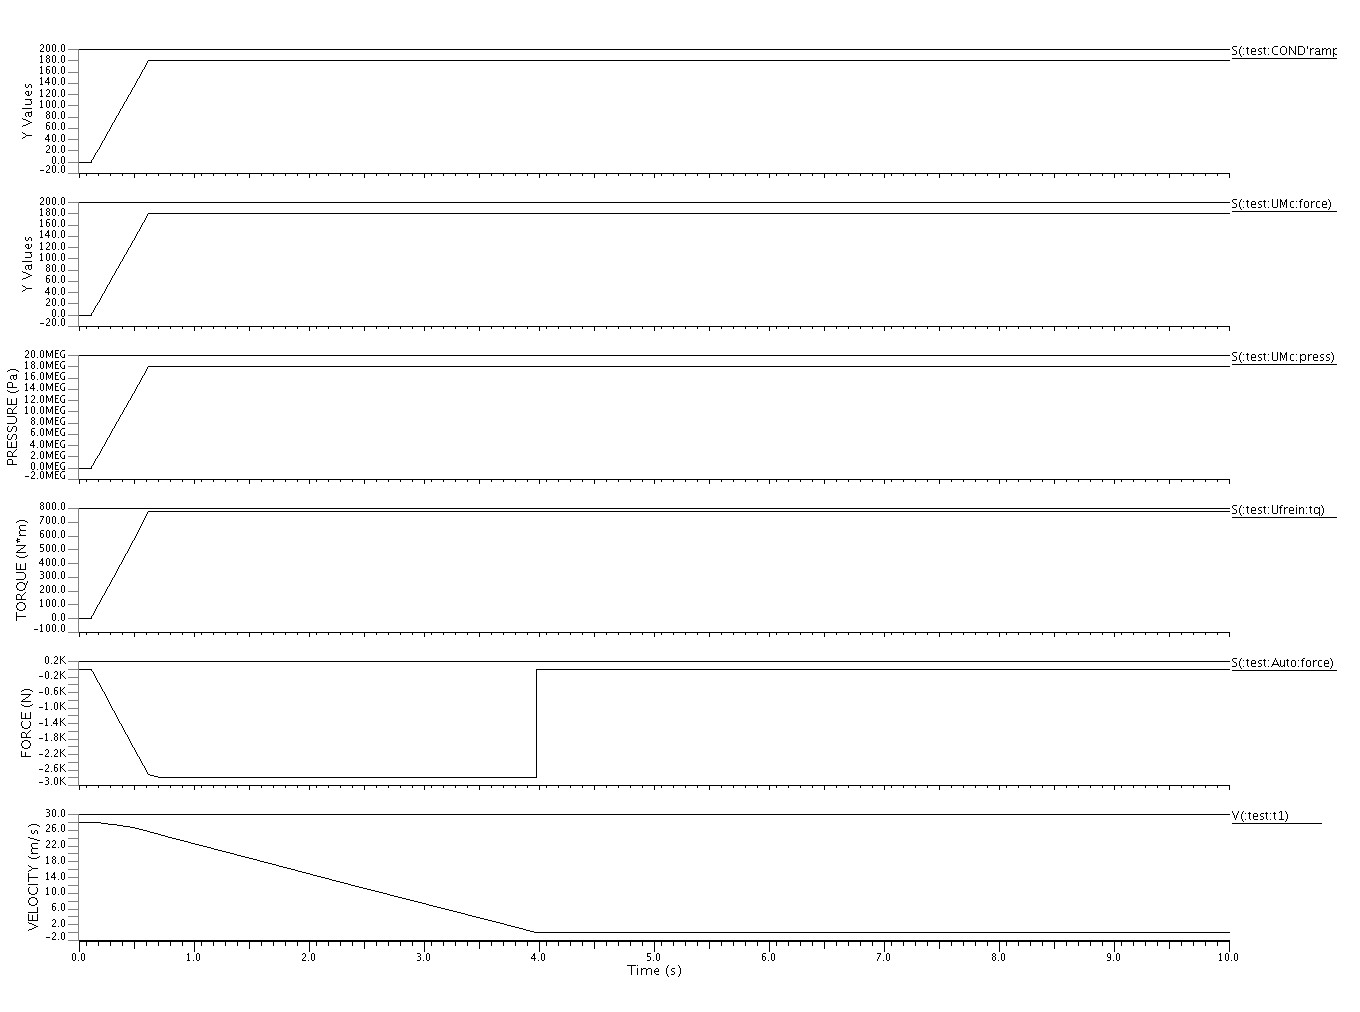
\includegraphics[width=\textwidth]{images/Instanciation_vehicule_roue_frein_Mc_rampe.jpg}
    \caption{Simulation avec temps de réaction sur le freinage}
\end{figure}

\newpage
\subsection{Modélisation du régulateur de pression}
a
\newpage